% 33-17(33쪽) — $y=3^{x}$ 의 그래프와 직선 $y=x$(원문 「오른쪽 그림」). 스캔 화질이 낮아 TikZ 로 다시 그림.
% 원문처럼 계단 모양 점선(축에 평행)만 넣는다. 라벨은 원문 것만: $y$축의 $1$, $x$축의 $\dfrac{1}{2}$·$a$·$b$, $\pt{O}$, 두 그래프 이름.
% 원문 그림도 눈금 없는 개략도다 — $b^{a}$(답)가 읽히지 않게 좌표값을 적지 않는다.
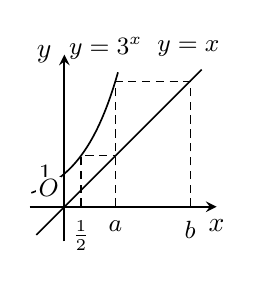
\begin{tikzpicture}[line width=0.6pt, x=0.42cm, y=0.42cm, >=stealth]
  \draw[densely dashed, line width=0.4pt] (0.5,0) -- (0.5,1.543) -- (1.543,1.543);
  \draw[densely dashed, line width=0.4pt] (1.543,0) -- (1.543,3.80) -- (3.80,3.80);
  \draw[densely dashed, line width=0.4pt] (3.80,0) -- (3.80,3.80);
  \draw[->, line width=0.7pt] (-1.05,0) -- (4.60,0) node[below=1pt] {$x$};
  \draw[->, line width=0.7pt] (0,-1.05) -- (0,4.60) node[left=1pt] {$y$};
  \draw[domain=-1.00:1.62, samples=90, smooth] plot (\x, {exp(0.866*\x)});
  \draw (-0.85,-0.85) -- (4.15,4.15);
  \node[anchor=east, font=\small] at (-0.08,1) {$1$};
  \node[anchor=north, font=\small] at (0.5,-0.12) {$\frac{1}{2}$};
  \node[anchor=north, font=\small] at (1.543,-0.12) {$a$};
  \node[anchor=north, font=\small] at (3.80,-0.12) {$b$};
  \node[anchor=south east, font=\small, fill=white, inner sep=0.8pt] at (-0.08,0.22) {$\pt{O}$};
  \node[anchor=south, font=\small] at (1.25,4.15) {$y=3^{x}$};
  \node[anchor=south, font=\small] at (3.75,4.25) {$y=x$};
\end{tikzpicture}
